% Primarily this section should be about scientific methods and theories you need to evaluate/compare/invent to solve your problems from 1.3.
% In some cases it may be ok to describe different technologies, but the purpose is to describe something and then draw a conclusion from that.
% Example, if you decide to discuss different databases, it may be for the purpose of selecting the best type for your implementation later on (based on for example data representation, scalability, speed, etc.).
% Optimally the problems in 1.3 are not solved by anyone else yet, in which case this section needs to describe how to solve them (new algorithms, mathematical approaches, etc.).
 
% This chapter can have a lot of sections (3.1, 3.2, 3.3, etc).

\section{Registers and Memory}
\label{sec:regmem}
% Primarily this section should be about scientific methods and theories you need to evaluate/compare/invent to solve your problems from 1.3.
% In some cases it may be ok to describe different technologies, but the purpose is to describe something and then draw a conclusion from that.
% Example, if you decide to discuss different databases, it may be for the purpose of selecting the best type for your implementation later on (based on for example data representation, scalability, speed, etc.).
% Optimally the problems in 1.3 are not solved by anyone else yet, in which case this section needs to describe how to solve them (new algorithms, mathematical approaches, etc.).
 
% This section can have a lot of subsections (3.1, 3.2, 3.3, etc).

The values of a computer program need to be temporary stored somewhere on the computer where they can easily be accessed while running the program.
The two main ways the computer can do this is to either store values in registers or in the memory.
Registers are very limited in space, and are very volatile.
Volatile in this case means that new values get written to the register often.
Thus, registers are good for storing values which are used many times in a very short amount of time.
Memory is much slower but has a lot more space.
Memory is thus much more useful for storing values that are not needed right now but will be needed in the future.


It is the compiler that decide when and if a variable will be stored in registers or memory.
The compiler decides this when compiling the computer program, which means the developer has usually very little control over where the values are stored.


Values stored in memory are either stored on the call stack or the heap.
The call stack holds all the arguments and variables for all the called functions that have not finished execution.
While the heap contain all the dynamically allocated values.


\subsection{Registers}
Computer registers are small memory spaces that are of fixed size.
These registers can store any type of data as long as it fits within the size limit of the registers.
Some registers are reserved for special use, one of the most important ones is the \acrfull{pc} register.
This register always holds the address of the next machine code instruction that will be executed.
Which of the registers that are reserved for special use is different depending on the processor.


\subsection{Call Stack}
\label{sec:callstack}
The call stack is a stack in the memory that has the arguments and variables of all the functions that have been called, and have not finished executing.
A stack is a data structure that consists of a number of elements that are stacked on top of each other and the only two operations available for a stack is push and pop.
The push operations will add an element on top of the stack, and the pop operation removes the top element of the stack.
Other key characteristics are that it is only the top element that can be accessed, thus to reach the lower elements, all the above elements needs to be popped.


Stack/call frames are the elements that make up the call stack.
Each stack frame contain the values of the arguments and variables for a function call, stack frames also contain a return address usually.
When a function is finished the return address is written to the \acrshort{pc} register, this makes the program jump to the return address.
The return address usually point back to the previous function, which called the function.
Also, when a function has finished executing, its stack frame will be popped/removed from the stack.
An example of a call stack and stack frames can be seen in figure \ref{fig:callstack}.
The values to the right in the figure are addresses, and they start with \emph{0x} because they are in hexadecimal.


\begin{figure}[h]
	\centering
	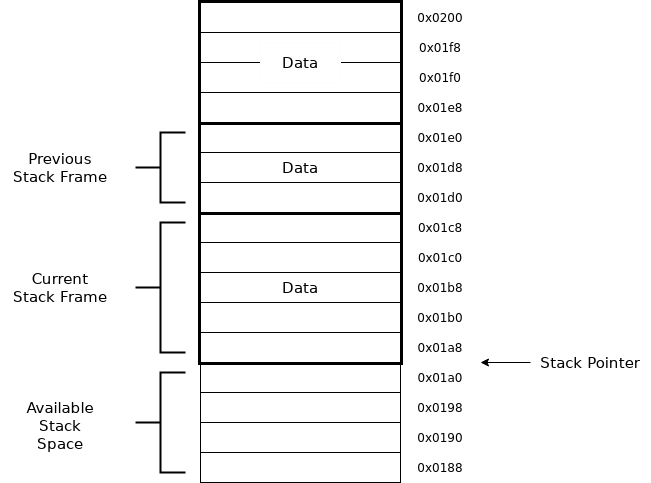
\includegraphics[width=1.0\textwidth]{call-stack.png}
	\caption{A visual example of how a stack and stack frames can look.}
	\label{fig:callstack}
\end{figure}


%\subsection{Heap}
%TODO



\section{Prologue and Epilogue Code}
% Primarily this section should be about scientific methods and theories you need to evaluate/compare/invent to solve your problems from 1.3.
% In some cases it may be ok to describe different technologies, but the purpose is to describe something and then draw a conclusion from that.
% Example, if you decide to discuss different databases, it may be for the purpose of selecting the best type for your implementation later on (based on for example data representation, scalability, speed, etc.).
% Optimally the problems in 1.3 are not solved by anyone else yet, in which case this section needs to describe how to solve them (new algorithms, mathematical approaches, etc.).
 
% This section can have a lot of subsections (3.1, 3.2, 3.3, etc).


Values in registers that need to be preserved during the execution of a subroutine will be pushed onto the call stack.
This is done by the prologue code that is executed at the start of the subroutine.
Then when the subroutine is finished executing, the stored register values are popped off the stack.
This is done by the epilogue code that is at the end of the subroutine.
The prologue and epilogue code is generated by the compiler.


Note that the prologue and epilogue code are not always continuous blocks of code that are in the beginning and end of a subroutine.
Instead sometimes the store and read operation are moved into the subroutine.
There are more of these special cases that the compiler does, and some that are hardware specific, to learn more about them see \cite{dwarf} page 126-127.



\section{Debugging}
% Primarily this section should be about scientific methods and theories you need to evaluate/compare/invent to solve your problems from 1.3.
% In some cases it may be ok to describe different technologies, but the purpose is to describe something and then draw a conclusion from that.
% Example, if you decide to discuss different databases, it may be for the purpose of selecting the best type for your implementation later on (based on for example data representation, scalability, speed, etc.).
% Optimally the problems in 1.3 are not solved by anyone else yet, in which case this section needs to describe how to solve them (new algorithms, mathematical approaches, etc.).
 
% This section can have a lot of subsections (3.1, 3.2, 3.3, etc).

Debugging refers to the process of finding and resolving errors, flaws, or faults in computer programs.
In computer science an error, flaw, or fault is often referred to as a bug.
Bugs are the cause for software behaving in an unexpected way.
Most bugs arise from badly written code, lack of communication between the developers and lack of programming knowledge.


There are multiple methods to debug computer programs.
One of the most common methods is testing, where some input is sent into the code, and then the result is compared to the expected result.
The amount of code being tested in a test can vary from just one function to the whole program.
Another method of debugging is to do a control flow analysis to see which order the instructions, statements, or function calls are done in.
There are a lot more methods to debug computer programs, but they all try to achieve the same thing.
And that is to give the programmer a deeper understanding of what is happening.


There is no better tool for understanding a program then a debugger.
That is because a debugger can display the state of a program and it give the program control of the execution.
Thus, a debugger enables a program to inspect every part of a program, this is especially true for modern debuggers, which have a lot more advance features.


\subsection{Debugger}
% Primarily this section should be about scientific methods and theories you need to evaluate/compare/invent to solve your problems from 1.3.
% In some cases it may be ok to describe different technologies, but the purpose is to describe something and then draw a conclusion from that.
% Example, if you decide to discuss different databases, it may be for the purpose of selecting the best type for your implementation later on (based on for example data representation, scalability, speed, etc.).
% Optimally the problems in 1.3 are not solved by anyone else yet, in which case this section needs to describe how to solve them (new algorithms, mathematical approaches, etc.).
 
% This section can have a lot of subsections (3.1, 3.2, 3.3, etc).


A debugger is a computer program that is used for testing and debugging other computer programs.
The program that is being debugged is often referred to as the target program.
The two main functionalities of a debugger, is firstly the ability to control the execution of the target program.
Secondly it is the ability to inspect the state of the target program.


Some of the most common ways a debugger can control a target program is by starting, stopping, stepping, and resetting the execution.
Starting the execution means that the target program continues the execution from the current stopped location, this also called continuing.
Stopping the target program or halting it, can often be done in two ways, the first is to stop the execution where it currently is, the other way is to set a breakpoint.
A breakpoint is a point in the code that if reached will stop the target program immediately.
Breakpoint are very useful for inspecting certain point in the code, while the other way of stopping is more used when the stopping location is unknown.
Stepping is the process of continuing the execution of the target program for only a moment, often just until the next source code line is reached, but there are many variants of stepping.
Lastly, resetting means that the target program will start execution from the beginning.


Most debugger display the state of the target program relative to the source code.
This means that if the target program has stopped, most debuggers will translate the location in the machine code it stopped on into the location of the source instruction from where the machine code instruction was generated from.
They also often let the user set the breakpoint in the source code, and translate that to the closest machine code instruction.
Other features most debuggers have is the ability to show a stack trace, variable values and to evaluate expression.
There are a lot more functionalities that a debugger can have, but these are some of the most common.



\section{DWARF}
\label{sec:dwarf}
% Primarily this section should be about scientific methods and theories you need to evaluate/compare/invent to solve your problems from 1.3.
% In some cases it may be ok to describe different technologies, but the purpose is to describe something and then draw a conclusion from that.
% Example, if you decide to discuss different databases, it may be for the purpose of selecting the best type for your implementation later on (based on for example data representation, scalability, speed, etc.).
% Optimally the problems in 1.3 are not solved by anyone else yet, in which case this section needs to describe how to solve them (new algorithms, mathematical approaches, etc.).
 
% This section can have a lot of subsections (3.1, 3.2, 3.3, etc).


% Explain what this section will contain.
This section will explain how the debug information format \acrfull{DWARF} version $4$ is structured, and how the different parts can be used to get debug information.
However, it will not explain every detail about the \gls{DWARF} format, because the \gls{DWARF} specification already does that.
Instead this section will focus on giving the reader an understanding of what type of information is stored in the \gls{DWARF} format.
And, to give some simple examples of how that information can be used to get the value of a variable for example.
Thus, we refer the reader to the \gls{DWARF} specification \cite{dwarf} for more details.


% Explain DWARF Sections
\subsection{Dwarf Sections}
% Primarily this section should be about scientific methods and theories you need to evaluate/compare/invent to solve your problems from 1.3.
% In some cases it may be ok to describe different technologies, but the purpose is to describe something and then draw a conclusion from that.
% Example, if you decide to discuss different databases, it may be for the purpose of selecting the best type for your implementation later on (based on for example data representation, scalability, speed, etc.).
% Optimally the problems in 1.3 are not solved by anyone else yet, in which case this section needs to describe how to solve them (new algorithms, mathematical approaches, etc.).
 
% This section can have a lot of subsections (3.1, 3.2, 3.3, etc).


% TODO: Explain DWARF Sections
The \gls{DWARF} format is divided into sections that all have different information and purpose.
These sections use offsets from the start of other sections to point to information in the other section, most of these offsets can be found in specific \gls{DWARF} attributes \ref{sec:dwarfattributes}.
The figure \ref{fig:dwarfsections} shows all the \gls{DWARF} sections and which ones point to each other.
All the \gls{DWARF} sections are stored in a \gls{elf} file, which is a binary file format that is divided into different sections.
The \gls{elf} format contain a table describe what each of its sections contain and where they begin and end.


%All of the sections are not in every version of \gls{DWARF} and are sometimes changed from version to version.
%Thus the following explanations are specific for \gls{DWARF} version $4$ but can sometimes also apply for other versions, checkout Appendix F in \cite{dwarf} for more information on the changes done from older versions.


\begin{figure}[h]
	\centering
	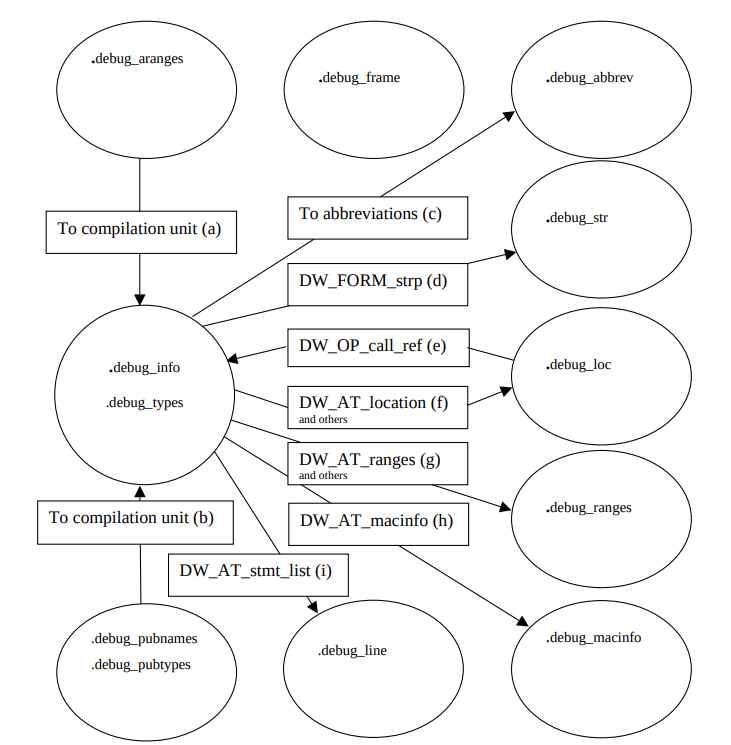
\includegraphics[width=0.9\textwidth]{dwarf-sections}
	\caption{Diagram of all the different \gls{DWARF} sections and their relations to each other.}
	\label{fig:dwarfsections}
\end{figure}


\subsubsection{\emph{.debug\_abbrev}}
The \gls{DWARF} section \emph{.debug\_abbrev} contain all the abbreviation tables which are used to translate abbreviation codes into its official \gls{DWARF} names.
These abbreviation codes are used for \gls{die} tags, \gls{die} attribute names and more.
To translate an abbreviation code one has to compare each entry until the one with the matching abbreviation code is found.
For further details we refer the reader to section $7.5.3$ in \cite{dwarf}.


\subsubsection{\emph{.debug\_aranges}}
The \gls{DWARF} section \emph{.debug\_aranges} is used to lookup compilation units using machine code addresses.
Each compilation unit has a range of machine code addresses that are the addresses that the compilation unit has information on.
These ranges consist of a start address followed by a length.
Thus, to find the compilation unit having the information about the current state, the user only needs to check if the current address is between the start address and the start address plus the length.
For further details we refer the reader to section $6.1.2$ in \cite{dwarf}.


\subsubsection{\emph{.debug\_frame}}
In the \gls{DWARF} section \emph{.debug\_frame} the information needed to virtually unwind the call stack is kept.
This section is completely self-contained, and is made up of two structures called \acrfull{cie} and \acrfull{fde}.
Virtually unwinding the call stack is complex, thus for further details we refer the reader section \ref{sec:stacktrace} in this document and section $6.4.1$ in \cite{dwarf}


\subsubsection{\emph{.debug\_info}}
Most of the information about the source code is stored in \glspl{die} which are low-level representation of the source code.
\glspl{die} have a tag that describes what it represents, an example tag is \emph{DW\_TAG\_variable} which means that the \gls{die} represents a variable from the source code.
All \glspl{die} are stored in trees, each one of the trees is a \gls{DWARF} compilation unit or a partial one.
The trees are structured the same as the source code, which makes it easy to relate the source code to the machine code.
The section \emph{.debug\_info} consist of a number of these \gls{DWARF} units, and some other debug information.
Thus, this is one of the most useful sections in \gls{DWARF}, because it is used to relate the state of the debug target and the source code, and vice versa.


\subsubsection{\emph{.debug\_line}}
The \gls{DWARF} section \emph{.debug\_line} holds the needed information to find the machine addresses which is generated from a certain line and column in the source file.
It is also used to store the source directory, file name, line number and column.
Then the \glspl{die} will store pointers to the source location information in the section \emph{.debug\_line} enabling the debugger to know the source location of a \gls{die}.
The section $6.2$ in \cite{dwarf} explains in more detail how this information is stored in the \emph{.debug\_line} section.


\subsubsection{\emph{.debug\_loc}}
The location of the variables values are stored in location lists, each entry in the list holds a number of operations that can be used to calculate the location of the value.
All the location lists are stored in the section \emph{.debug\_loc} and are pointed to by \glspl{die} in the \emph{.debug\_info} section.
These offsets are most commonly found in the attribute \emph{DW\_AT\_location} which is often present in \glspl{die} representing variables.
The relation between these two sections can be seen in figure \ref{fig:dwarfsections}.


\subsubsection{\emph{.debug\_macinfo}}
In the section \emph{.debug\_macinfo}, the macro information is stored.
It is stored in entries that each represents the macro after it has been expanded by the compiler.
These entries are also pointed to by \glspl{die} in the \emph{.debug\_info} section, and those pointers can be found in the attribute \emph{DW\_AT\_macinfo}.
This section is too complex, for further details we refer the reader to section $6.3$ in \cite{dwarf}.


\subsubsection{\emph{.debug\_pubnames} and \emph{.debug\_pubtypes}}
There are two sections for looking up compilation units by the name of functions, variables, types and more.
The first one is \emph{.debug\_pubnames} which is for finding functions, variables and objects, and the other one is for finding types, this section is called \emph{.debug\_pubtypes}.
Both of these are meant to be used for fast lookup of what unit the search information is located in.
For further details we refer the reader to section $6.1.1$ in \cite{dwarf}.


\subsubsection{\emph{.debug\_ranges}}
\Glspl{die} that have a set of addresses that are non-contiguous will have an offset to the section \emph{.debug\_ranges} instead of having an address range.
The offset points to the start of a range list that contain range entries which are used to know which of the machine code addresses the \gls{die} is active.
The \gls{DWARF} section \emph{.debug\_ranges} is used for storing these lists of ranges.
For further details we refer the reader to section $2.17$ in \cite{dwarf}.


\subsubsection{\emph{.debug\_str}}
The \gls{DWARF} section \emph{.debug\_str} is used for storing all the strings that is in the debug information.
An example of these strings are the names of the functions and variables.
These strings are found using an offset that are located in the attribute \emph{DW\_AT\_name}.
The attribute is found in the function and variable \glspl{die}, and the offset is in the form of \emph{DW\_FROM\_strp}.


\subsubsection{\emph{.debug\_type}}
The \gls{DWARF} section \emph{.debug\_type} is similar to section \emph{.debug\_info} in that it is also made up of units with each a tree of \glspl{die}.
The difference is that the \glspl{die} are a low-level representation of the types in the source code.



% Explain DWARF Unit
\subsection{Dwarf Compilation Unit}
% Primarily this section should be about scientific methods and theories you need to evaluate/compare/invent to solve your problems from 1.3.
% In some cases it may be ok to describe different technologies, but the purpose is to describe something and then draw a conclusion from that.
% Example, if you decide to discuss different databases, it may be for the purpose of selecting the best type for your implementation later on (based on for example data representation, scalability, speed, etc.).
% Optimally the problems in 1.3 are not solved by anyone else yet, in which case this section needs to describe how to solve them (new algorithms, mathematical approaches, etc.).
 
% This section can have a lot of subsections (3.1, 3.2, 3.3, etc).


% TODO: Explain DWARF Compilation Unit
When compiling a source program, the compiler will mostly generate one compilation unit for each project/library.
There are some cases when multiple partial compilation units will be generated instead.
The compilation units are store in the \gls{DWARF} section \emph{.debug\_info}.
These compilation units are structured the same as the source code, which makes it easy to relate between the debug target state and the source code.


%Finding the correct compilation unit can easily be done looking it up in the \gls{DWARF} section \emph{.debug\_aranges} using the current machine code address.
The first \gls{die} in the tree of the compilation unit will have the tag \emph{DW\_TAG\_compile\_unit}.
This \gls{die} has a lot of useful debug information about the source file, one being the compiler used and the version of it.
It also says which programming language the source file is written in as well as the directory and path of the source file.


A \gls{die} in the tree can have multiple children.
The relationship between the parent \gls{die}, and the children is that all the children belong to the parent \gls{die}.
An example of this is if there is a function \gls{die}, then the children of the function \gls{die} will be \glspl{die} that represent parameters and variables that are declared in that function.
Thus if the source code has a function declared in a function then one of the children to the first functions \gls{die} will be the second functions \gls{die}.
This makes it is easy for the debugger to know everything about a function by going through all of its children.



% TODO: Explain DWARF Die and Attributes
\subsection{Dwarf Debugging Information Entry}
% Primarily this section should be about scientific methods and theories you need to evaluate/compare/invent to solve your problems from 1.3.
% In some cases it may be ok to describe different technologies, but the purpose is to describe something and then draw a conclusion from that.
% Example, if you decide to discuss different databases, it may be for the purpose of selecting the best type for your implementation later on (based on for example data representation, scalability, speed, etc.).
% Optimally the problems in 1.3 are not solved by anyone else yet, in which case this section needs to describe how to solve them (new algorithms, mathematical approaches, etc.).
 
% This section can have a lot of subsections (3.1, 3.2, 3.3, etc).

% TODO: Explain DWARF Die

One of the most important data structures in the \gls{DWARF} format is the \gls{die}.
A \gls{die} is low level representation of a small part of the source code.
Some of the most common source code objects the \glspl{die} represent are functions, variables and types.
The \glspl{die} are found in a tree structure referred to as a \gls{die} tree.
Each \gls{die} tree will often represent a whole compile unit or a type from the source code.
The ones representing compile units are found in the \gls{DWARF} section \emph{.debug\_info}, while the ones representing type are found in the \gls{DWARF} section \emph{.debug\_type}.
The \glspl{die} representing types are often referred to as type \glspl{die}.


%The information stored in \glspl{die} are all in the form of \gls{DWARF} attributes.
%There are a lot of different attributes a \gls{die} can have, but they never have more then one of the same.
%The information in the attributes varies a lot depending on what attribute it is.


% TODO: Explain DWARF Attributes
\subsubsection{Dwarf Attribute}\label{sec:dwarfattributes}
% Primarily this section should be about scientific methods and theories you need to evaluate/compare/invent to solve your problems from 1.3.
% In some cases it may be ok to describe different technologies, but the purpose is to describe something and then draw a conclusion from that.
% Example, if you decide to discuss different databases, it may be for the purpose of selecting the best type for your implementation later on (based on for example data representation, scalability, speed, etc.).
% Optimally the problems in 1.3 are not solved by anyone else yet, in which case this section needs to describe how to solve them (new algorithms, mathematical approaches, etc.).
 
% This section can have a lot of subsections (3.1, 3.2, 3.3, etc).

% TODO: Explain DWARF Attribute

All the information stored in \glspl{die}, are stored in unique attributes, these attributes consists of a name and a value.
The name of the attribute is used to know what the value of the attribute should be used for.
It is also used to differentiate the different attributes.
All of the attributes names start with \emph{DW\_AT\_}, and then some name that describes the attribute, an example is the name attribute \emph{DW\_AT\_name}.
In the \gls{DWARF} file the name of the attributes will be abbreviated to their abbreviation code that can be decoded using the \emph{.debug\_abbrev} section.


\subsubsection{Example of a DIE}
An example of a \gls{die} can be seen in figure \ref{fig:dwarfdie}, the figure is a screenshot of the output from the program \emph{objdump} run on a \gls{elf} file.
The first line in the figure begins with a number $8$ which represents the depth in the \gls{die} tree this \gls{die} is located.
The next number is the current lines offset into this compile unit, all the other lines in the figure also start with their offset.
Then it says "Abbrev Number: 9" on the same line, this is an abbreviation code that translates to \emph{DW\_TAG\_variable}.
This tag means that the \gls{die} is representing a variable from the source code.


\begin{figure}[h]
	\centering
	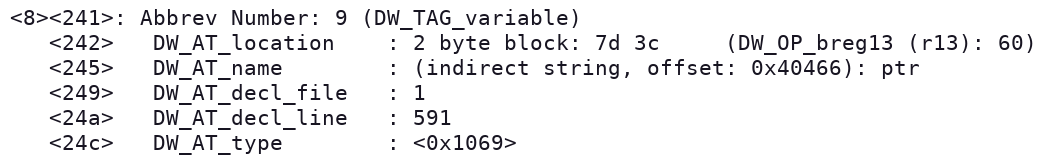
\includegraphics[width=1.0\textwidth]{dwarf-die.png}
	\caption{An example of a \gls{die} representing a variable named \emph{ptr}. This example is the output of the tool \emph{objdump} run on a \gls{DWARF} file.}
	\label{fig:dwarfdie}
\end{figure}


The attribute \emph{DW\_AT\_location} seen in figure \ref{fig:dwarfdie} has the information of where the variable is stored on the debug target.
The attribute \emph{DW\_AT\_name} has an offset into the \gls{DWARF} section \emph{.debug\_str} that the \emph{objdump} tool has evaluated to ``str'', this is the name of the variable.
Attributes \emph{DW\_AT\_decl\_file} and \emph{DW\_AT\_decl\_line} in the figure contain  offsets into the section \emph{.debug\_line}.
Those offsets can be evaluated to the source file path and line number that this \gls{die} is generated from.
Lastly the attribute \emph{DW\_AT\_type} contain an offset into the section \emph{.debug\_types}, that points to a type \gls{die} that has the type information for this variable.



% TODO: Explain evaluation
\subsection{Evaluate Variable}
\label{sec:evaluate-variable}
% Primarily this section should be about scientific methods and theories you need to evaluate/compare/invent to solve your problems from 1.3.
% In some cases it may be ok to describe different technologies, but the purpose is to describe something and then draw a conclusion from that.
% Example, if you decide to discuss different databases, it may be for the purpose of selecting the best type for your implementation later on (based on for example data representation, scalability, speed, etc.).
% Optimally the problems in 1.3 are not solved by anyone else yet, in which case this section needs to describe how to solve them (new algorithms, mathematical approaches, etc.).
 
% This section can have a lot of subsections (3.1, 3.2, 3.3, etc).

% TODO: Explain Evaluation of values

The process of evaluating the value of a variable is a bit complicated because there is a lot of variation.
Thus, to simplify the explanation, a simple example will be used to explain the main part of evaluating a variable.


Taking a look at the example in figure \ref{fig:subprogramexample} there is a function/subprogram \gls{die} with the name \emph{my\_function} (it is the \gls{die} with the tag \emph{DW\_TAG\_subprogram}).
The function has a parameter called \emph{val} which is the \gls{die} with the tag \emph{DW\_TAG\_formal\_parameter}, it is a child of the function \gls{die}.
Which means that it is a parameter to the function \emph{my\_function}.
It is this parameter \emph{val} that will be used as an example of how to evaluate a variable.


\begin{figure}[h]
	\centering
	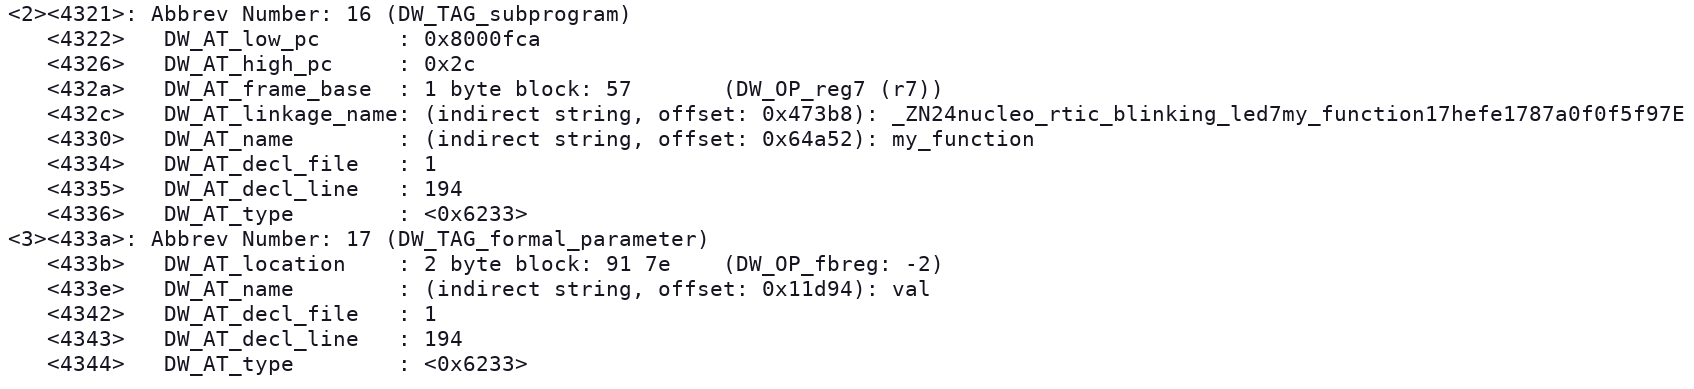
\includegraphics[width=1.0\textwidth]{subprogram-example.png}
	\caption{An example of a subprogram and parameter \gls{die}. This example is the output of the program \emph{objdump} run on a \gls{DWARF} file.}
	\label{fig:subprogramexample}
\end{figure}


Take note to the fact that the function \gls{die} called \emph{my\_function} has two attributes called \emph{DW\_AT\_low\_pc} and \emph{DW\_AT\_high\_pc}.
Those attributes describe the range of \gls{pc} values in which the function is executing.
There is also some other attributes in the example that will not be mentioned because they are not needed for determining the value of the attribute.


%Another important thing to note is that the example explained is a very simple one meaning that there is a lot more different \gls{DWARF} operation for finding the location of a variable and also a lot more different tags for the type \glspl{die}.
%All the various tags for type \glspl{die} requires a unique explanation to how it should be used thus the explanation of each one of them can be read about in the \gls{DWARF} specification \cite{dwarf}, the same goes for the different \gls{DWARF} operations.


\subsubsection{Finding Raw Value Location}
Examining the \gls{die} for the argument \emph{val} there is an attribute there called \emph{DW\_AT\_location}.
The value of that attribute is a number of operations, performing these operations will give the location of the variable.


In this example the operation in the \emph{DW\_AT\_location} attribute in figure \ref{fig:subprogramexample} is \emph{DW\_OP\_fbreg $-2$}.
That operation describes that the value is stored in memory at the \emph{frame base} minus $2$ (see \cite{dwarf} page 18).
The \emph{Frame base} is the address to the first variable in the functions stack frame (see \cite{dwarf} page 56).


Currently, the value of the \emph{frame base} is unknown, but the location of the \emph{frame base}  is described in the \emph{my\_function} \gls{die}.
The location of the \emph{frame base} is also described in a number of operations.
Those operations can be found under the attribute \emph{DW\_AT\_frame\_base}.
Looking at figure \ref{fig:subprogramexample}, the \emph{frame base} location is described with the operation \emph{DW\_OP\_reg7}.
The operation \emph{DW\_OP\_reg7} describe that the value is located in register $7$ (see \cite{dwarf} page 27).
Thus register $7$ needs to be read to get the value of the \emph{frame base}.


Now knowing the value of the \emph{frame base} the location of the parameter val can be calculated.
As mentioned previously, the location of parameter \emph{val} is the \emph{frame base} minus $2$.
Thus, the value of \emph{val} can be read from the memory at address of the \emph{frame base} minus $2$.
However, the value also has to be parsed into the type of \emph{val}, see section \ref{sec:parsingvalue} for how that is done.


\subsubsection{Parsing the Raw Value} \label{sec:parsingvalue}
Now the first problem with parsing the value of the parameter \emph{val} into the correct type is to know what type the parameter has, this is where the attribute \emph{DW\_AT\_type} comes in.
The value of the \emph{DW\_AT\_type} attribute points to a type \gls{die} tree, which describes the type of the \gls{die}.


The offset to the type \gls{die} of the parameter \emph{val} is $0x6233$, as can be seen in figure \ref{fig:subprogramexample}.
Finding that type \gls{die} is done by going to that offset in the \emph{.debug\_types} section.
The type \gls{die} for \emph{val} can be seen in figure \ref{fig:basetypeexample}, note that the offset of the \glspl{die} tag is the same as $6233$.
That type \gls{die} has the tag \emph{DW\_TAG\_base\_type} which means that it is a standard type that is built into most the languages (see \cite{dwarf} page 75).


\begin{figure}[h]
	\centering
	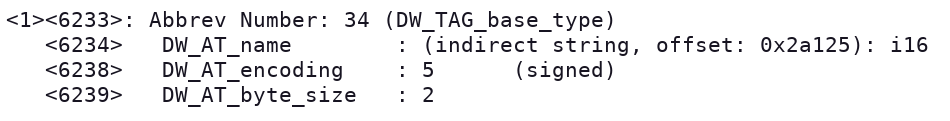
\includegraphics[width=1.0\textwidth]{basetype-example.png}
	\caption{An example of a base type \gls{die}. This example is the output of the program \emph{objdump} run on a \gls{DWARF} file.}
	\label{fig:basetypeexample}
\end{figure}


In this example the type \gls{die} has three attributes which are used to describe the type.
The first attribute is \emph{DW\_AT\_name}, it describes the name of the type.
In this case the name of the type is \emph{i16}, which can be seen in figure \ref{fig:basetypeexample}.
The next attribute is \emph{DW\_AT\_encoding}, this attribute describes the encoding of the type.
An encoding with the value $5$ means that the type is a signed integer \cite{dwarf}.
The different values for encoding are specified in the \gls{DWARF} specification \cite{dwarf}.
Now the last attribute is \emph{DW\_AT\_byte\_size}, it describes the size of the type in bytes.
A byte size of $2$ in this case means that the type is a $16$ bit signed integer.
Now that the type of \emph{val} is known the last step left to do is to parse the bytes of the value into a signed $16$ bit integer.



% TODO: Explain stacktrace
\subsection{Virtually Unwind the Call Stack}
\label{sec:stacktrace}
% Primarily this section should be about scientific methods and theories you need to evaluate/compare/invent to solve your problems from 1.3.
% In some cases it may be ok to describe different technologies, but the purpose is to describe something and then draw a conclusion from that.
% Example, if you decide to discuss different databases, it may be for the purpose of selecting the best type for your implementation later on (based on for example data representation, scalability, speed, etc.).
% Optimally the problems in 1.3 are not solved by anyone else yet, in which case this section needs to describe how to solve them (new algorithms, mathematical approaches, etc.).
 
% This section can have a lot of subsections (3.1, 3.2, 3.3, etc).

% TODO: Explain Unwinding call stack

Virtually unwinding the call stack is done by recursively unwinding a stack of \emph{subroutine activations}.
It is called virtual unwinding because the state of the debug target is not changed at any point during the unwinding.
Every subroutine in the call stack has an activation and a stack frame.
Because the activation often has the value of the stack pointer, the related stack frame is also known.
Thus, successfully unwinding all the \emph{subroutine activations} will result in complete understanding of the state of the call stack.


The debug information needed to unwind activations are stored in the \gls{DWARF} section \emph{.debug\_frame}.
That section is made up of two data structures, one is called \gls{fde}.
A \gls{fde} contains a table used for unwinding registers and the \gls{cfa} of an activation.
The other data structure is called \gls{cie}, it contains information that is shared among many \glspl{fde}.
The relevant \gls{cie} and \gls{fde} to an activation can be found using the code location where it is stopped.


Unwinding the stack of activation is done by first evaluating the values of the top activation, see section \ref{sec:subact} to learn how that is done.
It starts with the top activation because there is too little information known of the other activations.
Next step is to find the \gls{cie} and \gls{fde} that contain debug info on the next activation.
When those are known the values of the next activation can be evaluated as described in section \ref{sec:subact}.
This is then repeated for the rest of the activations.


% ###############################################
\subsubsection{Subroutine Activation} \label{sec:subact}
A \emph{subroutine activation} contain information on a subroutine call/activation.
Each \emph{subroutine activation} contain a code location within the subroutine, it is the location where the subroutine stopped.
The reason for stopping could be that a breakpoint was hit, it was interrupted by an event, or it could be a location where it made a call to the next subroutine.


The address of the stopped code location is easily found using the stack pointer of the above activation in the activation stack.
That is because the return address of the above activation is the stopped code location of the current activation.
The return address is almost always stored on the stack thus it can easily be read if the stack pointer is known.
This works for all activations except for the top activation, where the current \gls{pc} value is the stopped code location.


An activation also describes the state of some registers where it stopped.
Those are the registers that are preserved thanks to the prologue and epilogue code of the subroutine.
The rest of the registers are unknown because they have been written over, which makes them impossible to recover.


The activations are identified by there \gls{cfa} value. 
The \gls{cfa} is the value of the stack pointer in the previous stack frame.
Note that the \gls{cfa} is not the same value as the stack pointer when entering the current \emph{call frame} (see \cite{dwarf} page 126).


Both the values of the \gls{cfa} and the preserved register can be restored using tables located in the \gls{DWARF} section \emph{.debug\_frame}.
For further details, the reader is referred to section \ref{sec:evalcfa}.



% ###############################################
\subsubsection{Unwinding CFA and Registers} \label{sec:evalcfa}
The tables in the \glspl{fde} contains virtual unwinding rules for a subroutine.
These virtual unwinding rules are used to restore the values of registers and the \gls{cfa}.


The first column in the tables contains code addresses.
Those addresses are used to identify the code location that all the virtual unwinding rules on that row applies for.
Next column is special because it contains the virtual unwinding rules for \gls{cfa}.
The rest of the columns contain the virtual unwinding rules for registers $0$ to $n$, where $n$ is the last registry.
See figure \ref{fig:stacktracetable} for a visual of how the tables are structured.


\begin{figure}[h]
	\centering
	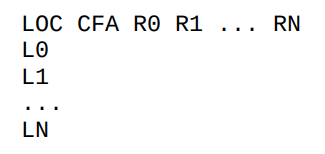
\includegraphics[width=0.5\textwidth]{stacktrace-table.png}
	\caption{This is how the table for reconstructing the \gls{cfa} and registers looks like. \emph{LOC} means that it is the column containing the code locations for $0$ to $N$. The column with \gls{cfa} has the virtual unwinding rules for \gls{cfa}. The rest of the column \emph{R0} to \emph{RN} holds all the virtual unwinding rules for the register $0$ to $N$.}
	\label{fig:stacktracetable}
\end{figure}


There are a number of different virtual unwinding rules, the ones for the registers are called register rules.
Some of them are easy to use such as the register rule \emph{undefined}.
This rule means that it is impossible to unwind that register.
Other ones require some calculations such as the register rule \emph{offset(N)}, where the \emph{N} is a signed offset.
This rule means that the register value is stored at the \gls{cfa} address plus the offset $N$.
All the rules can be read about in the \gls{DWARF} specification \cite{dwarf} on page 128.


Unwinding a register is done by first finding the correct row.
That is done by finding the closest address that is less than the search one.
Next step is to evaluate the new value using the register rule on the row, then go to the next row in the table, and repeat but with the new value.
Repeat until there are no more rows.
That is how to use the table to unwind a register.
